%%%%%%%%%%%%%%%%%%%%%%%%%%%%%%%%%%%%%%%%%%%%%%%%%%%%%%%%%%%%%%%%%%%%%%%%%%
%
% HST_GO_proposal_cy34.tex (Use only for General Observer and Snapshot
% proposals. Use HST_AR_proposal_cy34.tex for Archival Research and Theory
% proposals; use HST_DD_proposal_cy34.tex for GO/DD proposals).
%
% HUBBLE SPACE TELESCOPE
% PHASE I OBSERVING PROPOSAL TEMPLATE
% FOR CYCLE 34 and beyond
%
% Version 3.6; November 2025
%
% Guidelines and assistance
% =========================
% Hubble Call for Proposals Announcement Web Page:
%
% https://hst-docs.stsci.edu/
%
% Please contact the STScI Help Desk if you need assistance with any
% aspect of proposing for and using HST at
% https://stsci.service-now.com/hst.
%
%%%%%%%%%%%%%%%%%%%%%%%%%%%%%%%%%%%%%%%%%%%%%%%%%%%%%%%%%%%%%%%%%%%%%%%%%%%

% The template begins here. Please do not modify the font size from 12 point.

\documentclass[12pt]{article}
\usepackage[letterpaper]{geometry}
\usepackage{hstproposaltemplate_cy34}
\usepackage{graphicx}
\usepackage{natbib}
\usepackage{amsmath}

\begin{document}

% 1. SCIENTIFIC JUSTIFICATION
\justification % Do not delete this command.

\subsection*{Background and Motivation}

Type~Ia supernovae (SNe~Ia) serve as the cornerstone of modern cosmology,
providing the first direct evidence for the accelerated expansion of the
Universe \citep{Riess1998, Perlmutter1999}. As precision cosmology enters
the era of Stage~IV surveys, systematic uncertainties in SNe~Ia distance
measurements are becoming the dominant limitation. One subtle but
potentially significant systematic is dust extinction by intergalactic
medium (IGM) dust along the sightline to each supernova.

\citet{Menard2010} demonstrated statistically that intergalactic dust
introduces a redshift-dependent dimming and reddening of background
sources, with a mean rest-frame $B$-band opacity of $A_B \gtrsim 0.03$
magnitudes at $z = 0.5$. This signal was detected via cross-correlation of
quasar colors with foreground galaxy positions over scales from 20~kpc to
several Mpc, and it implies that IGM dust introduces a systematic bias in
the SNe~Ia Hubble diagram that grows with redshift. The associated dust
resides primarily in \ion{Mg}{2} absorbing clouds around galaxies:
\citet{MenardFukugita2012} measured the cosmic dust density in \ion{Mg}{2}
absorbers to be $\Omega_{\rm dust} \sim 2 \times 10^{-6}$, comparable to
the amount of dust in galactic disks, and with a dust-to-gas ratio
consistent with an outflow origin. Most recently, \citet{Menard2026}
have provided updated theoretical predictions for the IGM dust signal
expected in individual SNe~Ia sightlines, motivating the direct
spectroscopic test we propose here.

Despite these compelling statistical detections, no study has yet obtained
\emph{direct spectroscopic proof} that IGM dust along individual SNe~Ia
sightlines is associated with intervening \ion{Mg}{2} absorption. The
connection between photometric reddening of SNe~Ia and the predicted
spectroscopic signature has never been tested on a per-object basis. We
propose to close this gap with a proof-of-concept non-disruptive Target of
Opportunity (ToO) program using the Cosmic Origins Spectrograph (COS) on
HST.

\subsection*{Scientific Goals}

This program has two primary science goals:

\begin{enumerate}
\item \textbf{Direct detection of IGM \ion{Mg}{2} absorption in SNe~Ia
  spectra.} By obtaining UV spectroscopy of anomalously reddened SNe~Ia in
  the COSMOS Deep Drilling Field (DDF), we will search for \ion{Mg}{2}
  $\lambda\lambda$2796, 2803 absorption at the redshifts of foreground
  galaxies identified along each sightline. A detection of \ion{Mg}{2}
  absorption correlated with the photometric color excess $\Delta E(B-V)$
  would constitute the first per-object spectroscopic confirmation of the
  IGM dust hypothesis of \citet{Menard2010, Menard2026}.

\item \textbf{Search for Damped Lyman-$\alpha$ (DLA) systems.} For
  sightlines where a foreground galaxy places the Lyman-$\alpha$ line
  within the COS G130M bandpass, we will search for the characteristic
  damping wings of DLA systems ($N_{\rm HI} \geq 2 \times 10^{20}$
  cm$^{-2}$). A DLA detection along a reddened SNe~Ia sightline would
  provide a direct measure of the neutral hydrogen column associated with
  IGM dust, enabling a constraint on the dust-to-gas ratio of the
  absorbing medium.
\end{enumerate}

\begin{figure}[h]
\centering
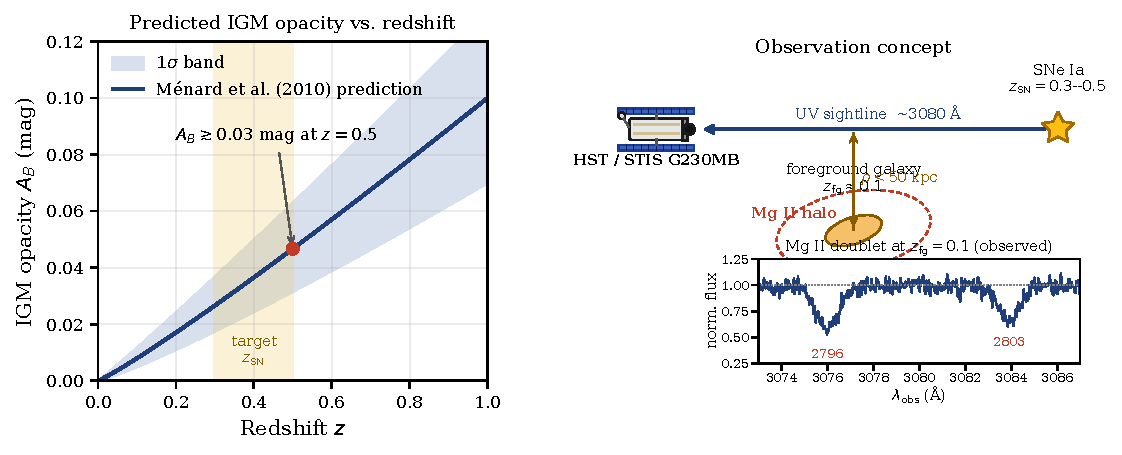
\includegraphics[width=0.95\textwidth]{figures/fig1_science_case.pdf}
\caption{
  \textbf{Left:} The predicted IGM opacity as a function of redshift
  from \citet{Menard2010}, showing the rest-frame $B$-band extinction
  $A_B$ growing to $\sim$0.03--0.05 mag by $z \sim 0.5$. This
  redshift-dependent effect biases SNe~Ia cosmological parameter
  estimates if uncorrected.
  \textbf{Right:} Schematic of the observation concept. A LSST-discovered
  SNe~Ia at $z_{\rm SN} = 0.3$--0.45 (background source) is observed with
  COS G185M. \ion{Mg}{2} absorption from a foreground galaxy at
  $z_{\rm fg} < z_{\rm SN}$ within impact parameter $\rho < 200$~kpc
  imprints a characteristic doublet on the UV spectrum, directly tracing
  the dust responsible for the photometric reddening detected by LSST.
}
\label{fig:science}
\end{figure}

\subsection*{Why HST/COS is Uniquely Required}

The \ion{Mg}{2} $\lambda\lambda$2796, 2803 doublet at $z_{\rm fg} =
0.1$--0.5 falls at observed wavelengths of 3080--4200~\AA\ --- deep in the
near-UV, inaccessible to ground-based telescopes. COS G185M is the only
instrument in existence capable of detecting these absorption lines at the
required spectral resolution ($R \sim 16{,}000$--20{,}000) with sufficient
UV sensitivity to observe SNe~Ia at $z \sim 0.3$--0.45 (peak UV magnitude
$m_{\rm UV} \sim 20.5$--21.5 AB). No ground-based facility can access
wavelengths below $\sim$3200~\AA\ at the required sensitivity. This program
is therefore uniquely enabled by HST.

\subsection*{Target Field: COSMOS Deep Drilling Field}

We focus exclusively on the COSMOS Deep Drilling Field
($10^{\rm h}00^{\rm m}$, $+02\degr12'$). The COSMOS field offers
unparalleled advantages for this program:

\begin{itemize}
\item \textbf{LSST/Rubin DDF priority:} COSMOS receives double the visit
  allocation of other DDFs ($\sim$40{,}000 visits over 10 years) and
  reaches 10-year survey depth within the first 3 years of operations
  \citep{GrisDDF2024}. This maximizes the early SNe~Ia discovery rate
  during the first HST Cycle.

\item \textbf{Extraordinary ancillary data:} The COSMOS2020 photometric
  redshift catalog provides photo-$z$ measurements with $\sigma_z/(1+z)
  \sim 0.01$ for $\sim$10$^6$ galaxies to $i \sim 25$~AB
  \citep{Weaver2022}. The zCOSMOS and C3R2 spectroscopic surveys provide
  secure spectroscopic redshifts for foreground galaxies at $z < 1$.
  HST-ACS morphology measurements enable precise dDLR calculations for all
  host galaxies.

\item \textbf{Contemporaneous spectroscopic support:} The PFS/Subaru
  survey will obtain $\sim$20{,}000 host galaxy spectroscopic redshifts in
  the COSMOS field contemporaneously with LSST operations, eliminating the
  need for pre-trigger spectroscopy.
\end{itemize}

Based on the LSST Science Book estimate of $\sim$2{,}500 SNe~Ia per DDF
per year and the COSMOS double-visit allocation, we conservatively expect
150--250 SNe~Ia per year at $z = 0.3$--0.45 in the COSMOS field, of which
6--10 will satisfy all selection criteria (see Section~2) per year ---
providing a robust target pool for 5--7 non-disruptive ToO triggers per
HST Cycle.

%%%%%%%%%%%%%%%%%%%%%%%%%%%%%%%%%%%%%%%%%%%%%%%%%%%%%%%%%%%%%%%%%%%%%%%%%%%

% 2. DESCRIPTION OF THE OBSERVATIONS
\describeobservations % Do not delete this command.

\subsection*{Overview}

We request 34 HST orbits for a non-disruptive Target of Opportunity
program to obtain COS/NUV G185M UV spectroscopy of 5--7 SNe~Ia in the
COSMOS Deep Drilling Field, triggered within 3 weeks of discovery by the
LSST/Rubin Observatory. Each target requires 4--5 HST orbits, fitting
comfortably within the 34-orbit small-program limit.

\subsection*{Target Selection Cascade}

The richness of the COSMOS field allows us to be highly selective,
pre-qualifying targets through a five-stage filter cascade before any HST
time is committed (Figure~\ref{fig:selection}).

\textbf{Stage 1 --- LSST discovery and alert.}
We monitor the LSST COSMOS DDF alert stream in real time. Rubin issues
photometric alerts within 60~s of each detection. We consider all
transients classified as SNe~Ia by LSST photometric classifiers with
light-curve parameters consistent with a normal thermonuclear event.

\textbf{Stage 2 --- Photometric redshift filter ($z = 0.30$--$0.45$).}
We require the SNe~Ia host galaxy to have a COSMOS2020 photo-$z$ in the
range $z = 0.30$--0.45, confirmed to $\sigma_z/(1+z) < 0.02$. This window
ensures that \ion{Mg}{2} $\lambda$2796 from a foreground absorber at any
$z_{\rm fg} < z_{\rm SN}$ falls within the COS G185M peak sensitivity
region (observed 1700--2100~\AA\ with CENWAVE 1900), and that the SNe~Ia
UV continuum at rest $\sim$2700~\AA\ reaches $m_{\rm UV} \lesssim 21.5$~AB
--- bright enough for S/N~$= 10$ per resolution element in 4--5 HST
orbits.

\textbf{Stage 3 --- Large dDLR cut (host dust rejection).}
The Directional Light Radius \citep[dDLR;][]{Sullivan2006} measures the
angular separation between a SNe~Ia and its host galaxy normalized by the
ellipsoidal half-light radius of the host in the direction of the SN.
We require $\rm dDLR > 3$, meaning the SNe~Ia lies more than 3 host
half-light radii from the nucleus in its direction. This efficiently
rejects SNe~Ia embedded in dusty spiral disks, ensuring that any observed
color excess is more plausibly of IGM rather than host-ISM origin. The
required morphological parameters (semimajor axis, position angle,
Petrosian radius) are available from the HST-ACS COSMOS morphology catalog
for all galaxies to $i \sim 26$~AB. This cut reduces the candidate pool by
$\sim$60\% while retaining those events best suited to our science goal.

\textbf{Stage 4 --- Foreground galaxy sightline search.}
For each remaining candidate, we search the COSMOS2020 and zCOSMOS
catalogs for a galaxy at $z_{\rm fg} < z_{\rm SN}$ within a projected
impact parameter $\rho \leq 200$~kpc of the SNe~Ia sightline. The
\ion{Mg}{2} absorber-galaxy catalog MAGIICAT \citep{Nielsen2013}
demonstrates a well-established 8$\sigma$ anti-correlation between
\ion{Mg}{2} equivalent width and impact parameter, with a covering
fraction of $\sim$70\% for $W_0(2796) > 0.3$~\AA\ at $\rho < 50$~kpc
\citep{Dutta2020}. We tier targets by impact parameter (highest priority:
$\rho < 50$~kpc; medium priority: $\rho = 50$--150~kpc) and require
$z_{\rm fg}$ to place \ion{Mg}{2} $\lambda$2796 within the G185M
bandpass. Sightlines where the foreground galaxy also places Ly$\alpha$
within the COS G130M range are flagged as DLA candidates.

\textbf{Stage 5 --- Anomalous photometric reddening.}
We require the LSST SALT3 light-curve fit to show a residual color excess
$\Delta E(B-V) \geq 0.03$~mag relative to the standard SNe~Ia template
color. Because Stage~3 already eliminates host-dust events, a residual
excess at this stage is statistically more likely to be of IGM origin ---
precisely the signal predicted by \citet{Menard2010, Menard2026}. This
filter biases the sample toward sightlines where the \ion{Mg}{2} signal is
most likely to be detectable, maximizing scientific return.

After applying all five stages, we expect 6--10 COS-ready targets per
year in the COSMOS field. We trigger on the best 5--7 per Cycle, ranked
by (1) foreground galaxy impact parameter and (2) $\Delta E(B-V)$ excess.

\begin{figure}[h]
\centering
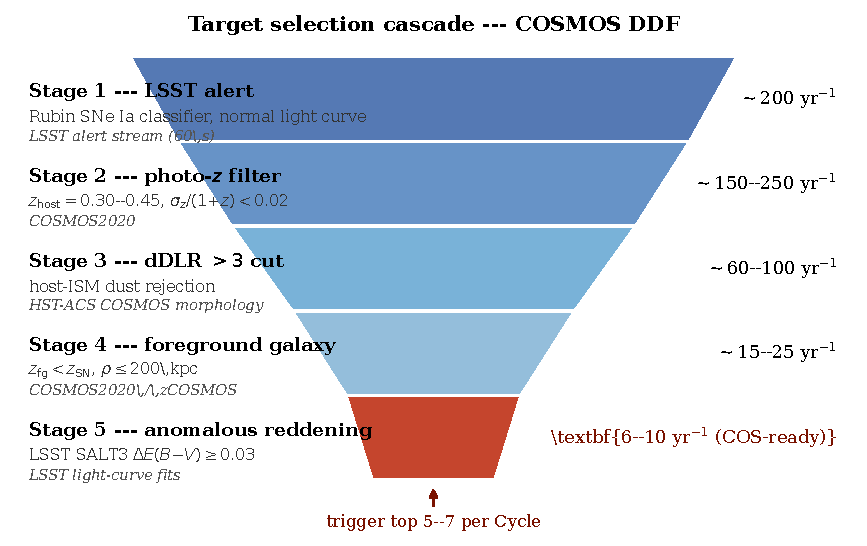
\includegraphics[width=0.88\textwidth]{figures/fig2_target_selection.pdf}
\caption{
  Target selection cascade. Starting from $\sim$200 SNe~Ia per year at
  $z = 0.3$--0.45 in the COSMOS DDF, five successive filters reduce the
  pool to 6--10 COS-ready targets per year. We trigger on the top 5--7
  per HST Cycle as non-disruptive ToO observations. The yield at each
  stage is shown, along with the COSMOS data asset used. The dDLR $> 3$
  cut (Stage~3) is the key discriminator that isolates IGM reddening
  from host-galaxy dust contamination.
}
\label{fig:selection}
\end{figure}

\subsection*{Instrument Configuration}

All observations use COS in spectroscopic mode with the Primary Science
Aperture (PSA):

\begin{itemize}
  \item \textbf{Grating:} G185M, CENWAVE 1900~\AA.\ This setting provides
    continuous wavelength coverage from $\sim$1700--2100~\AA\ across
    NUV stripes A, B, C, covering \ion{Mg}{2} $\lambda\lambda$2796, 2803
    at $z_{\rm fg} = 0.10$--0.52 and the COS G185M peak effective area
    region.

  \item \textbf{Spectral resolution:} $R \sim 16{,}000$--20{,}000
    ($\Delta v \sim 15$--20 km~s$^{-1}$ per resolution element),
    sufficient to resolve the \ion{Mg}{2} doublet and measure rest
    equivalent widths $W_0(2796) \geq 0.3$~\AA\ at the required
    significance.

  \item \textbf{FP-POS:} All 4 positions will be used to mitigate fixed
    pattern noise and detector artifacts, following standard COS
    observing practice.

  \item \textbf{Target acquisition:} ACQ/IMAGE with MIRRORA followed by
    spectroscopic observation. Total acquisition overhead: $\sim$6~min
    per visit.

  \item \textbf{Bright object protection:} All targets will be screened
    against COS bright-object limits using the STScI ETC prior to
    triggering. SNe~Ia at $z = 0.3$--0.45 at peak ($m_{\rm UV} \sim
    20.5$--21.5~AB) are well below NUV bright-object limits.
\end{itemize}

\subsection*{Exposure Time and Orbit Budget}

We adopt a science goal of S/N~$\geq 10$ per COS resolution element at
the wavelength of \ion{Mg}{2} $\lambda$2796 from the foreground absorber.
This is sufficient to detect absorption with rest equivalent width
$W_0(2796) \geq 0.3$~\AA\ at $>3\sigma$ significance, covering the full
range of \ion{Mg}{2} absorbers associated with galaxy halos
\citep{Nielsen2013}. The COS detector has no read noise (photon counter),
so S/N scales cleanly as $\sqrt{t}$.

Table~\ref{tab:orbits} summarizes the orbit allocation per target as a
function of redshift. At our optimal target redshift of $z_{\rm SN} =
0.35$, the SNe~Ia UV continuum reaches $m_{\rm UV} \approx 21.0$~AB,
requiring $\sim$10{,}500~s of on-source science time (S/N~$= 10$, G185M,
continuum flux). With $\sim$44~min of on-source time per orbit after
accounting for guide star acquisition (6.5~min), reacquisition (6.5~min
per subsequent orbit), target acquisition (6~min), and instrument
overheads (5~min first exposure + 2~min subsequent), each target requires
4 orbits.

\begin{table}[h]
\centering
\caption{Orbit allocation per SNe~Ia target (S/N~$= 10$, COS G185M).}
\label{tab:orbits}
\begin{tabular}{lcccc}
\hline\hline
$z_{\rm SN}$ & $m_{\rm UV}$ (AB) & Science exp.\ (s) & Orbits/target & Targets in 34 orbits \\
\hline
0.30 & 20.5 & 6{,}600  & 3 & 11 \\
0.35 & 21.0 & 10{,}560 & 4 & 8  \\
0.40 & 21.4 & 14{,}400 & 5 & 6  \\
0.45 & 21.9 & 21{,}120 & 6 & 5  \\
\hline
\end{tabular}
\end{table}

\noindent
Our baseline program observes \textbf{6 targets at $z_{\rm SN} =
0.30$--0.40} (mixed, depending on trigger availability), using
\textbf{$\sim$24--30 orbits}, with 4--10 orbits held as contingency for
targets at slightly higher redshift or for repeat observations in the
event of a scheduling conflict. The total request of \textbf{34 orbits}
accommodates 5--7 targets across the redshift range with full scheduling
flexibility.

Each visit is structured as a multi-orbit visit to allow guide star
reacquisition between orbits and maximize on-source efficiency. The four
FP-POS positions are distributed across exposures within each visit.

\subsection*{Non-Disruptive Target of Opportunity Designation}

This program is designated as a \textbf{non-disruptive Target of
Opportunity}. Triggers will be submitted only when a qualifying LSST SNe~Ia
is identified through the automated five-stage selection pipeline. We
anticipate 5--7 triggers per Cycle, each submitted within 3 weeks of
SNe~Ia discovery while the UV flux remains near peak brightness ($\pm$2
weeks from $B$-band maximum). The non-disruptive designation means that
HST observations will be scheduled within the normal scheduling queue
without interrupting ongoing observations, consistent with the estimated
trigger frequency of fewer than one per month. No prior approval is
required for individual triggers beyond the initial TAC approval of this
program.

\subsection*{Expected Outcomes}

With 6 sightlines observed, we expect $\sim$0.4--0.6 strong \ion{Mg}{2}
detections ($W_0 > 0.3$~\AA) based on the absorber incidence rate $dN/dz
\sim 0.25$ for strong systems at $z \sim 0.3$--0.5
\citep{MenardFukugita2012}. By selecting sightlines with known foreground
galaxies at $\rho < 200$~kpc, we boost the expected detection rate to
$\sim$1--2 absorbers per 6 targets \citep{Nielsen2013}. Even a single
detection with a correlated photometric $\Delta E(B-V)$ excess would
constitute the first direct spectroscopic proof of the IGM dust hypothesis
for individual SNe~Ia. A non-detection over 6 sightlines would itself
provide a 2$\sigma$ constraint on the Ménard dust prediction --- a
scientifically valuable result. DLA detection would be a significant bonus,
directly measuring the neutral hydrogen column of the absorbing system.

%%%%%%%%%%%%%%%%%%%%%%%%%%%%%%%%%%%%%%%%%%%%%%%%%%%%%%%%%%%%%%%%%%%%%%%%%%

% 3. ANALYSIS PLAN
% Not required for a standard GO program --- section omitted.

%%%%%%%%%%%%%%%%%%%%%%%%%%%%%%%%%%%%%%%%%%%%%%%%%%%%%%%%%%%%%%%%%%%%%%%%%%

% 4. SPECIAL REQUIREMENTS
\specialreq % Do not delete this command.

This program requests \textbf{non-disruptive Target of Opportunity}
status. The following special requirements apply:

\begin{itemize}
  \item \textbf{ToO trigger window:} Each trigger must be executed within
    3 weeks of SNe~Ia discovery by LSST. The SNe~Ia UV flux is brightest
    within $\pm$2 weeks of $B$-band maximum; observations outside this
    window will result in insufficient S/N.

  \item \textbf{Multi-orbit visits:} Each target requires a multi-orbit
    visit of 3--6 consecutive or near-consecutive orbits, as detailed in
    Table~\ref{tab:orbits}. Standard guide star reacquisition between
    orbits applies.

  \item \textbf{FP-POS 1--4:} All four focal-plane offset positions must
    be used to eliminate fixed pattern noise on the COS NUV MAMA detector,
    as required for faint-source continuum spectroscopy.

  \item \textbf{Bright object screening:} Each ToO target must be
    screened against COS NUV bright-object limits using the STScI ETC
    prior to trigger submission. Only targets satisfying all COS safety
    limits will be triggered.

  \item \textbf{No scheduling windows:} As a non-disruptive ToO, no
    specific scheduling windows are required. Triggers will be placed in
    the scheduling queue and executed at the next available opportunity
    within the 3-week constraint.
\end{itemize}

%%%%%%%%%%%%%%%%%%%%%%%%%%%%%%%%%%%%%%%%%%%%%%%%%%%%%%%%%%%%%%%%%%%%%%%%%%

% 5. COORDINATED OBSERVATIONS
\coordinatedobs % Do not delete this command.

This program is scientifically coordinated with the LSST/Rubin Observatory
COSMOS Deep Drilling Field survey, which provides the SNe~Ia discovery
alerts and multi-band photometric light curves used for target selection.
No formal coordination agreement with Rubin is required, as LSST alert
data will be publicly available within 60 seconds of each detection through
the Rubin alert broker network.

The PFS/Subaru spectroscopic survey of the COSMOS field is expected to
provide host galaxy spectroscopic redshifts contemporaneously with LSST
operations and will be used where available to confirm photo-$z$
estimates. No formal ToO coordination with Subaru is required.

No Director's Discretionary or pre-approved HST observations in the
COSMOS field overlap with our science goals. The COS UV spectroscopy
we propose has not been obtained for any LSST-discovered transient to
date.

%%%%%%%%%%%%%%%%%%%%%%%%%%%%%%%%%%%%%%%%%%%%%%%%%%%%%%%%%%%%%%%%%%%%%%%%%%

% 6. JUSTIFY DUPLICATIONS
% No duplications with existing HST programs. Section omitted.

%%%%%%%%%%%%%%%%%%%%%%%%%%%%%%%%%%%%%%%%%%%%%%%%%%%%%%%%%%%%%%%%%%%%%%%%%%

\subsection*{References}

\begin{description}
  \item \citet{Dutta2020}: Dutta, R.\ et al.\ 2020, MNRAS, 499, 5054
  \item \citet{GrisDDF2024}: Gris, P.\ et al.\ 2024, A\&A (arXiv:2405.10781)
  \item \citet{MenardFukugita2012}: M\'enard, B.\ \& Fukugita, M.\ 2012,
    ApJ, 754, 116
  \item \citet{Menard2010}: M\'enard, B., Kilbinger, M., \& Scranton, R.\
    2010, MNRAS, 406, 1815
  \item \citet{Menard2026}: M\'enard, B.\ et al.\ 2026, ApJ, 1000, 313
  \item \citet{Nielsen2013}: Nielsen, N.~M.\ et al.\ 2013, ApJ, 776, 114
  \item \citet{Perlmutter1999}: Perlmutter, S.\ et al.\ 1999, ApJ, 517, 565
  \item \citet{Riess1998}: Riess, A.~G.\ et al.\ 1998, AJ, 116, 1009
  \item \citet{Sullivan2006}: Sullivan, M.\ et al.\ 2006, AJ, 131, 960
  \item \citet{Weaver2022}: Weaver, J.~R.\ et al.\ 2022, ApJS, 258, 11
\end{description}

\end{document} % End of proposal. Do not delete this line.
% Everything after this command is ignored.
